\documentclass[wabun2025.tex]{subfiles}
\begin{document}
\section{方法}
\subsection{変数}
本章の中の式では、電気素量、電子質量、ボーア半径、プランク定数の値がそれぞれ1と
なる原子単位系(atomic units, a.u.)を用いる。

本報告で用いる変数は表\ref{tab:variables}に示すとおりである。

\begin{table}[ht]
    \centering
    \caption{本章で用いる変数}
    \begin{tabular}{cc}
        変数 & 説明 \\
        \hline
        $d$ & 空間の次元数 \\
        $\nb$ & 座標レジスタのビット数 \\
        $L$ & シミュレーション領域の一辺の大きさ \\
        $\deltar$ & 位置座標空間の格子間隔 \\
        $\deltak$ & 波数空間の格子間隔 \\
        $\deltat$ & 時間発展の時間刻み \\
        $\chij$ & 格子点$j$の離散化座標
    \end{tabular}
    \label{tab:variables}
\end{table}

\subsection{シミュレータと計算モデルの概要}
本研究で評価対象とするシミュレータ回路の構成と、シミュレーション対象とする
水素原子モデルについて説明する。

\subsubsection{波動関数の格納方法}
本研究で開発したシミュレータ回路生成プログラムは、複数電子と複数原子核からなるモ
デルの回路を生成することが可能であるが、本報告で扱うモデルは単一水素原子のモデル
であり、原子核は座標系の原点で静止しているものとして扱う。空間の次元数は1次元と2
次元を対象とする。

位置基底 $\{\ket{j}\}$ は離散格子点 $\{\chij\}$ に対応する直交基底とし、
\begin{equation}
\braket{i|j}=\delta_{ij}
\end{equation}
を満たすものとする。

この場合、位置座標表示での状態ベクトル$\ketPsiRS$ は、離散化座標 $\chij$を持つ格
子点$j$での波動関数の振幅$\Psi_j=\Psi(\chij\deltar)$とを用いて、
\begin{equation}
\ketPsiRS = \sum_{j}\Psi_j\ket{j}
\end{equation}
で表される。、一方波数表示での状態ベクトル $\ketPsiKS$ は、
平面波基底関数$W_{\ell}(\bm{r})=e^{i\bm{k}_{\ell}\cdot\bm{r}}/\sqrt{L^d}$ と
その基底の波数を持つ波動関数の成分$\tilde{\Psi}_{\ell}$とを用いて、
\begin{equation}
\Psi(\bm{r})=\sum_{\ell} \tilde{\Psi}_{\ell}W_{\ell}(\bm{r})\leftrightarrow
\ketPsiKS = \sum_{\ell}\tilde{\Psi}_{\ell}\ket{\ell}
\end{equation}
と表される。

電子のみを量子的に扱う系における1ステップの時間発展回路 $\Thetae$ の作用
は、Suzuki-Trotter分解に基づいて1ステップ分の時間発展演算を行うことである。 1次
の式を用いた場合には、これは
\begin{align}
\ket{\Psi(t+\deltat)}
 &= e^{-iH\deltat/\hbar}\ket{\Psi(t)} \notag \\
 &\approx \Thetae \ket{\Psi(t)} \label{eq:circuit-eval-theta-e}\\
 &= \Thetaep\QFT\Thetaek\QFTdagger\ket{\Psi(t)}\\
    \Thetaep&=e^{-i\Hep\deltat/\hbar}\\
    \Thetaek&=e^{-i\Hek\deltat/\hbar}
\end{align}
と表される。

時間発展演算子の運動エネルギー項は波数表示において、位置エネルギー項は位置座標表
示表示においてそれぞれ計算する。原子単位系を用い、原子核の位置を座標系の原点に取
るとハミルトニアンの運動エネルギー項 $\Hek$ と位置エネルギー項 $\Hep$ は一次元と
二次元のモデルでそれぞれ以下のように表される。

\begin{align}
   \HekOneD(\bm{k}) = -\frac{(\hbar\kx)^2}{2}, \qquad &
   \HepOneD(\bm{r}) = -\frac{1}{\abs{x}} \label{eq:HkHp1D}\\
   \HekTwoD(\bm{k}) = -\frac{(\hbar\kx)^2 + (\hbar\ky)^2}{2}, \qquad &
   \HepTwoD(\bm{r}) = -\frac{1}{\sqrt{x^2+y^2}} \label{eq:HkHp2D}
\end{align}

シミュレータ回路はqubitの初期化回路$\PsiSD$と時間発展回路から構成され、時間発展回路
は１ステップの時間発展回路$\Thetae$を必要なステップ数繰り返したものである。初期化
回路の作用は、qubitに波動関数の初期値を格納することである。
\begin{equation}
\ket{\Psi(t=0)} = \PsiSD \ket{0}
\end{equation}
これには初期波動関数の準備回路を用いる\cite[Sec. 2.2]{takahashi2024.doi:10.1021/acs.jctc.4c00708}。

\subsubsection{計算モデル}
本報告での評価では水素原子の一次元と二次元のモデルの時間に依存しないシュレディンガー
方程式の解を用いる。時間に依存しないシュレディンガー方程式の解は時間に依存する
シュレディンガー方程式の定常解として得られる。そのため、この解を初期値として時間
発展させた場合には、振幅の絶対値は時間に依存せず、位相のみが時間に依存することに
なる。位相変化の速さも解の固有値として得られるため、計算結果の評価に使うことがで
きる。

\begin{equation}
H\psi(\bm{r})=E\psi(\bm{r})
\end{equation}
の解が複数の固有値$E_n$と固有関数$\psi_n(\bm{r})$を持つとき、すなわち
\begin{equation}
H\psi_n(\bm{r})=E_n\psi_n(\bm{r}),\quad n=1,2,\ldots
\end{equation}
となる時、固有値$E_n$に対応する固有関数を初期値とした系の波動関数は
\begin{equation}
\Psi_n(\bm{r},t)=\psi_n(\bm{r})\exp\left(-\frac{iE_nt}{\hbar}\right)
\end{equation}
のように表される。シミュレーションの結果を比較する基準としてこの式を用いる。

シミュレーション対象とする一次元のモデルと二次元のモデルそれぞれの解析解を以下に
示す。

一次元のモデルに関しては、Loudonによる一次元のモデルの解析解を用いる
\cite{Loudon1959.10.1119/1.1934950}。Loudonによれば、基底状態となる主量子数$n=0$
の解はデルタ関数となる。$n>0$の解に関しては偶関数の解と奇関数の解が示されてい
る。本論文ではこのうち、フーリエ変換で扱うことができる奇関数の解を取り上げる。量
子数 $n\in{1,2,\ldots}$ の奇関数の解を $\psi_n^{\mathrm{1D}}$ で表す。
\begin{equation}
\psi_n^{\mathrm{1D}}(x)=\sqrt{\frac{2}{a_0^3n^5(n!)^2}}
x\exp\left(-\frac{\abs{x}}{na_0}\right)L_n^1\left(\frac{2\abs{x}}{na_0}\right)
\end{equation}
ここで、$L_n^k$は、Laguerreの陪多項式である。このエネルギー固有値は量子数
$n\in{1,2,\ldots}$ を用いて
\begin{equation}
    E_n^{\mathrm{1D}}=-\frac{\hbar^2}{2\melec a_0^2 n^2}
\end{equation}
で与えられる。評価には量子数$n=1$の波動関数$\psi_1^{\mathrm{1D}}$とその固有値
$E_1^{\mathrm{1D}}$は次のようになる:
\begin{align}
\psi_1^{\mathrm{1D}}(x)&=\sqrt{2}e^{-\abs{x}} x
\label{eq:psi1D1-wave-function}\\
E_1^{\mathrm{1D}}&=-\frac{1}{2}
\label{eq:psi1D1-energy}
\end{align}

$\psi_1^{\mathrm{1D}}$ の位置座標表示と波数表示を図\ref{fig:initial-wavefunction-1d}に示す。

\begin{figure}[ht]
    \centering
    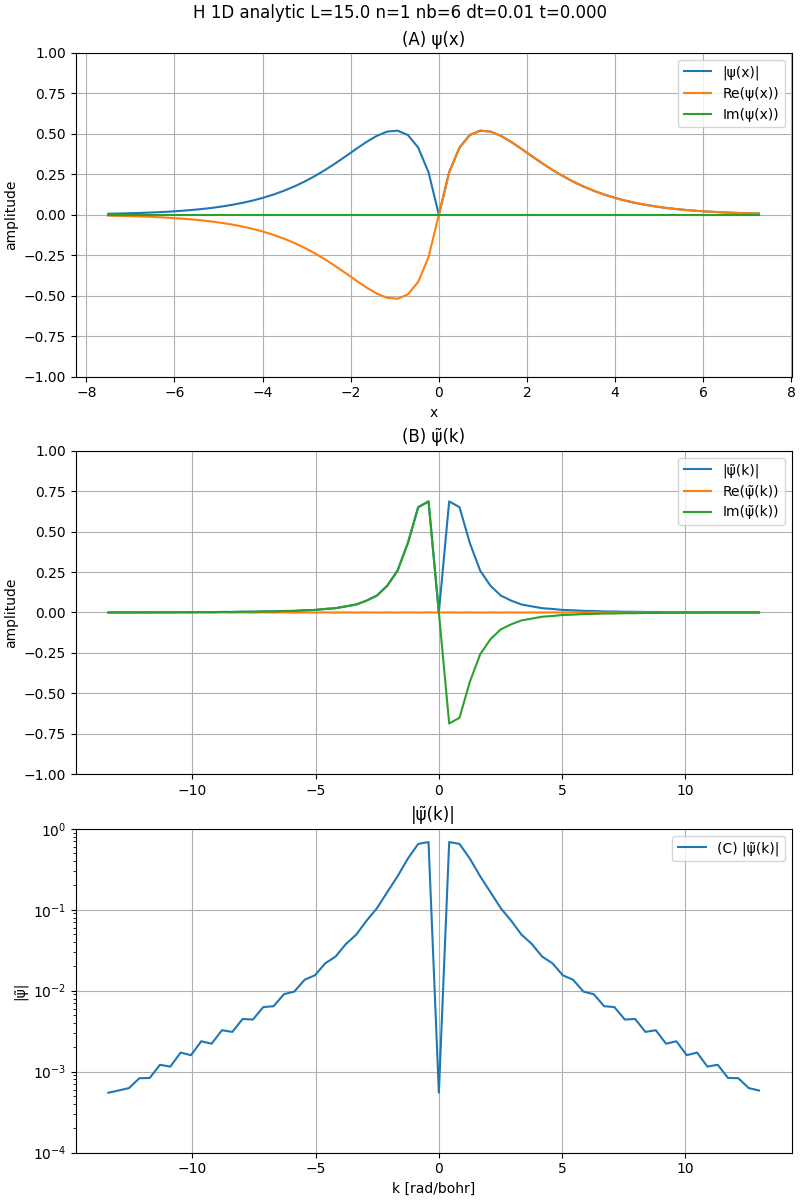
\includegraphics[width=0.6\textwidth]{paper2025_figs/analytic1D/t_00.000.png}
    \caption{1次元モデルの波動関数 $\PsiOneD_1$ の例}
    \label{fig:initial-wavefunction-1d}
    \begin{flushleft}\small

        6ビット分解能での $\PsiOneD_1$ の値(式\eqref{eq:psi1D1-wave-function})。
        (A)はreal-spaceでの波動関数の振幅である。(B)はk-spaceでの波動関数の振幅
        である。(C)はk-spaceの振幅の対数スケール表示である。

    \end{flushleft}
\end{figure}

二次元のモデル$\psi_{n,\ m}^{\mathrm{2D}}$は、Parfittによる解析解を用いる
\cite{Parfitt2002.10.1063/1.1503868}。このモデルは、クーロンポテンシャル
$-1/\sqrt{x^2+y^2}$の下で運動する電子を二次元平面上に拘束したモデルである。波動
関数は二つの量子数 $n\in\{0,\ldots\}, m\in\{-n,\ldots,0,\ldots,n\}$ をパラメータ
として持つ。
\begin{equation}
\psi_{n,\ m}^{\mathrm{2D}}(r,\ \theta)=
\sqrt{\frac{q_0^3(n-\abs{m})!}{\pi(n+\abs{m})!}}(2q_0r)^{\abs{m}}
e^{-q_0r}L_{n-\abs{m}}^{2\abs{m}}(2q_0r)e^{im\theta}
\end{equation}
ここで $q_0=1/(n+1/2)$ である。このエネルギー固有値は量子数$n\in\{0,\ldots\}$を用いて
\begin{equation}
E_n^{\mathrm{2D}}=-\frac{1}{2(n+1/2)^2}
\end{equation}
で与えられる。評価には基底状態$\psi_{0,0}^{2D}$と励起状態$\psi_{1,0}^{2D}$と
$\psi_{1,1}^{2D}$を用いる。これら２つの波動関数と固有値はそれぞれ以下のように表
される。
\begin{align}
\psi_{0,0}^{\mathrm{2D}}(r,\theta)&=\sqrt{\frac{8}{\pi}}e^{-2r}
\label{eq:psi2D00-wave-function}\\
E_0^{\mathrm{2D}}&=-2
\label{eq:psi2D00-energy}\\
\psi_{1,0}^{\mathrm{2D}}(r,\theta)&=\sqrt{\frac{8}{27\pi}}(1-\frac{4}{3}r)e^{-\frac{2}{3}r} 
\label{eq:psi2D10-wave-function}\\
\psi_{1,1}^{\mathrm{2D}}(r,\theta)&=\frac{8}{9\sqrt{3\pi}}re^{-\frac{2}{3}r+i\theta}
\label{eq:psi2D11-wave-function}\\
E_1^{\mathrm{2D}}&=-\frac{2}{9}\simeq -0.2222
\label{eq:psi2D10-energy}
\end{align}

$\psi_{0,0}^{\mathrm{2D}}, \psi_{1,0}^{\mathrm{2D}}, \psi_{1,1}^{\mathrm{2D}}$
の位置座標表示と波数表示をそれぞれ図\ref{subfig:initial-wavefunction-2d-0-0},
\ref{subfig:initial-wavefunction-2d-1-0}, \ref{subfig:initial-wavefunction-2d-1-1}  に
示す。

\begin{figure}[ht]
    \centering
    \begin{subfigure}{.45\columnwidth}
        \centering
        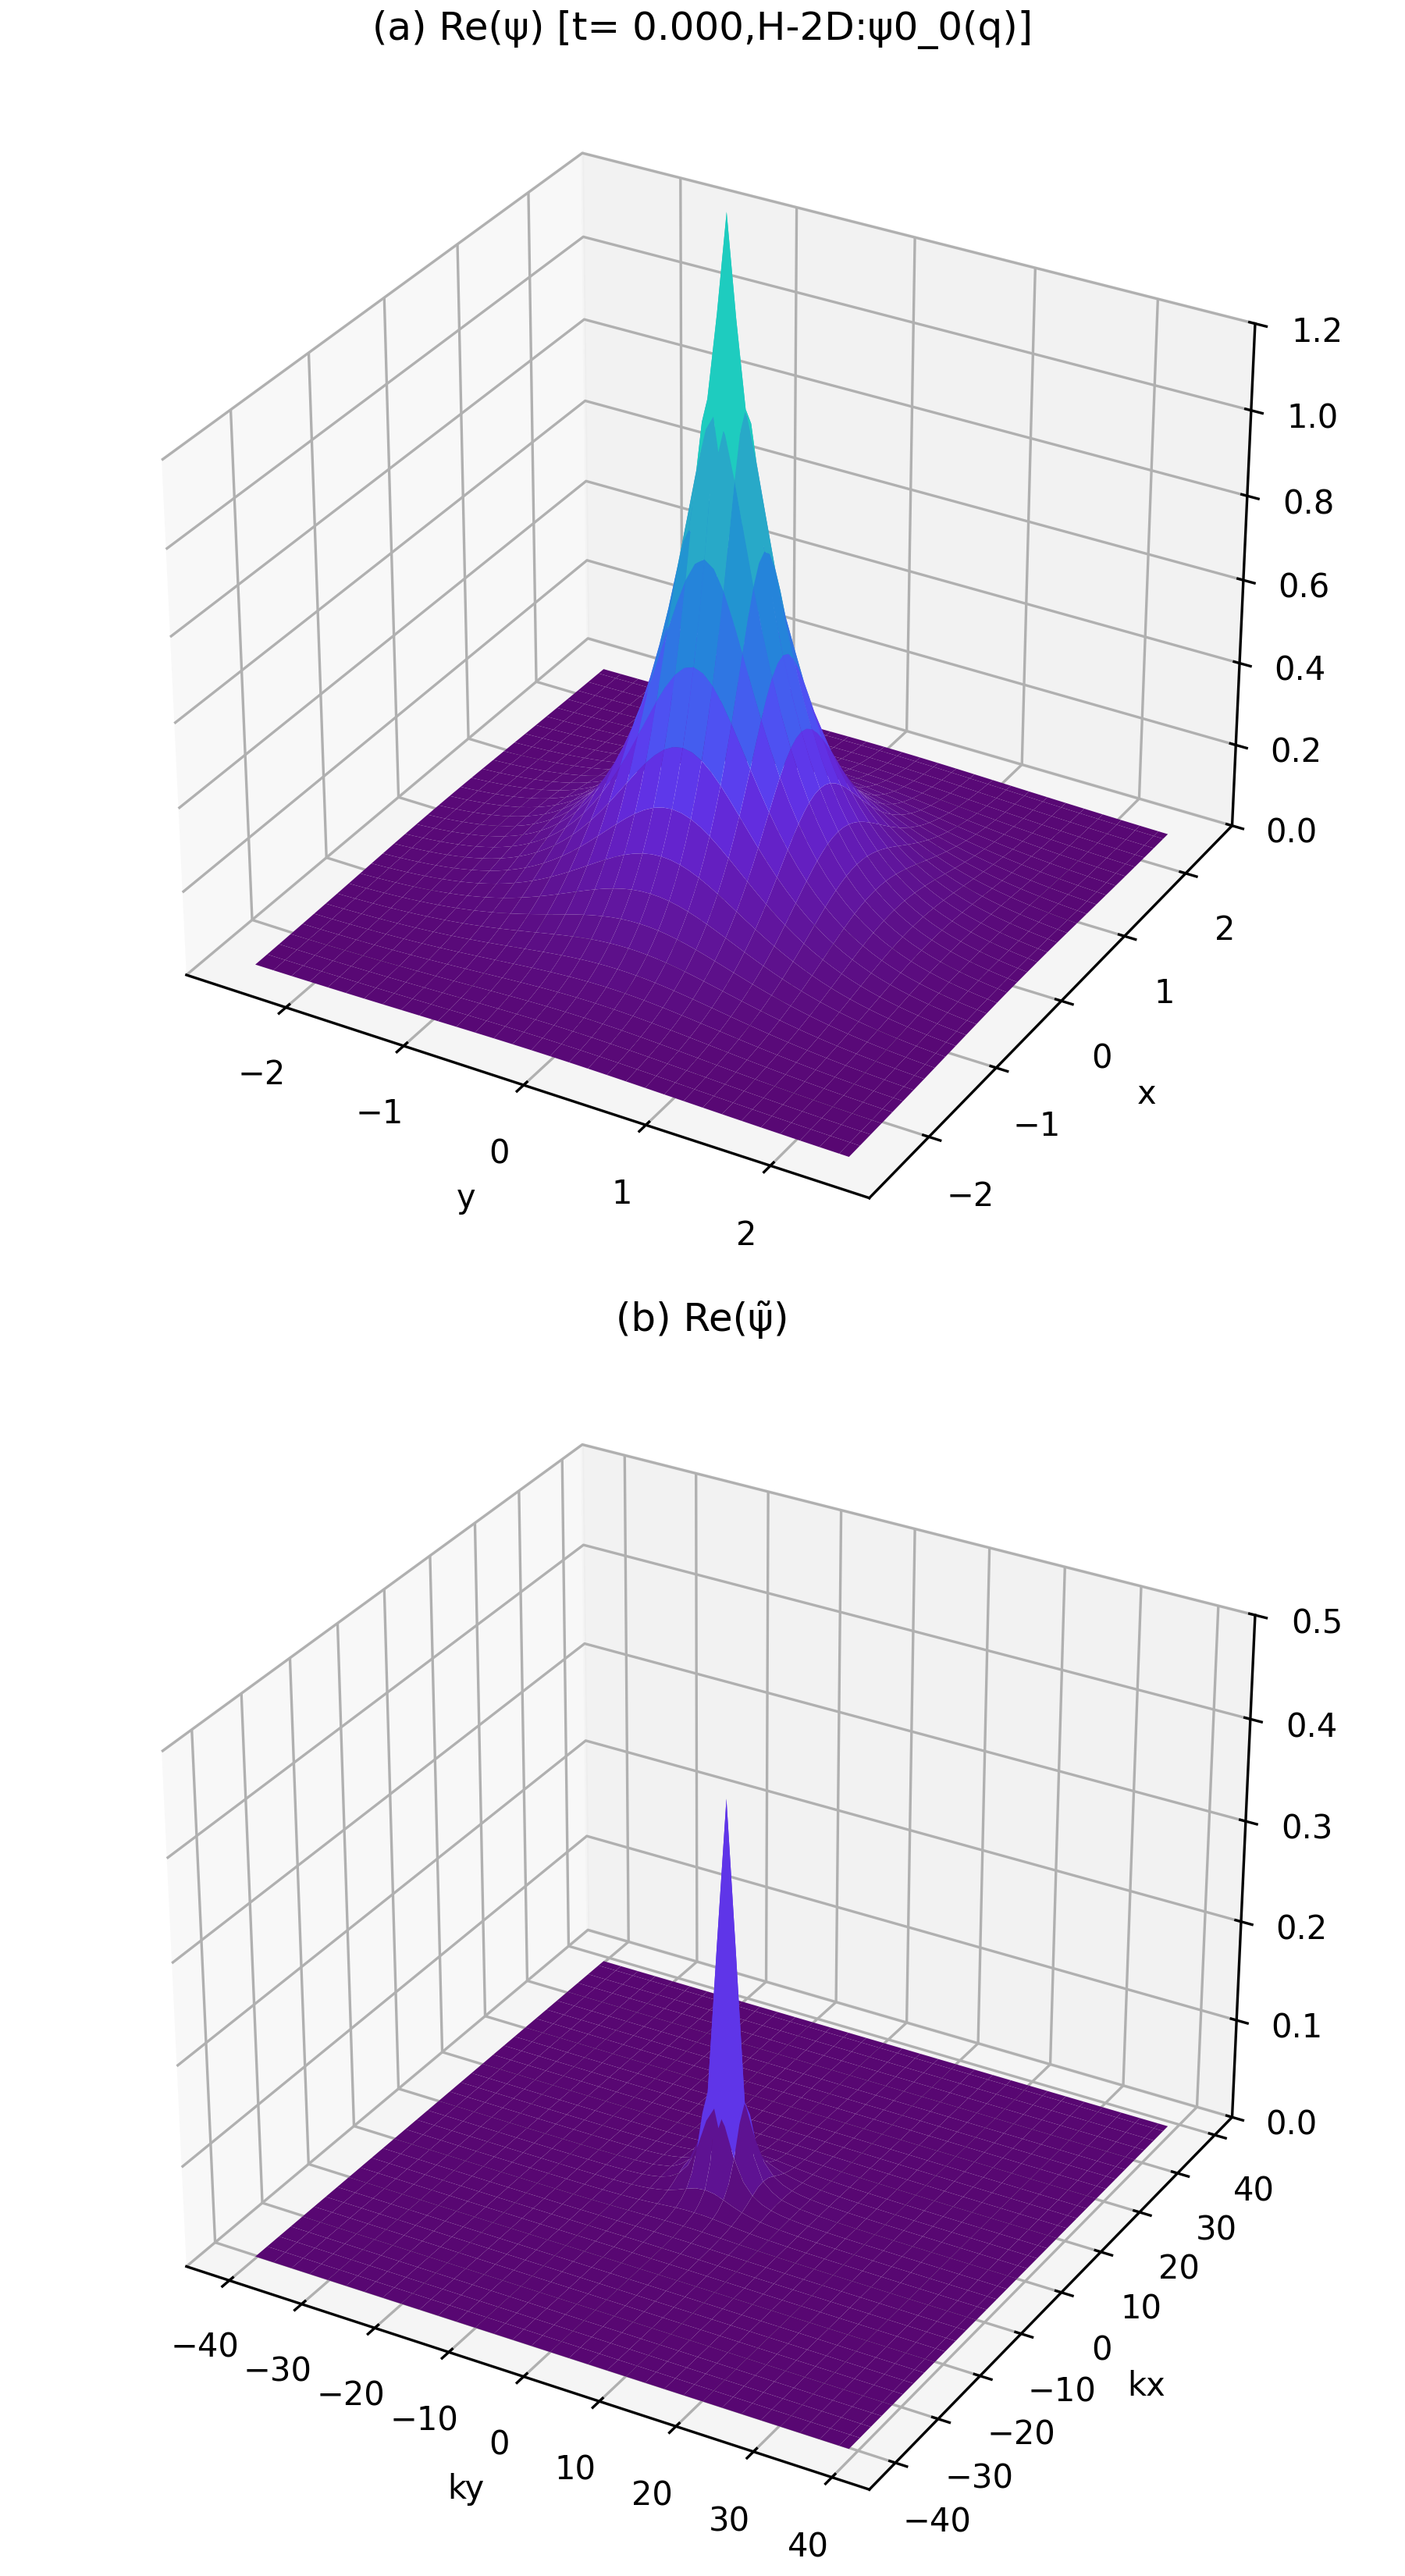
\includegraphics[width=1\columnwidth]{paper2025_figs/classic2D/6b_n0_m0/t_00.000_3d-qp.png}
        \caption{波動関数 $\PsiTwoD_{0,0}$}
        \label{subfig:initial-wavefunction-2d-0-0}
    \end{subfigure}
    \begin{subfigure}{.45\columnwidth}
        \centering
        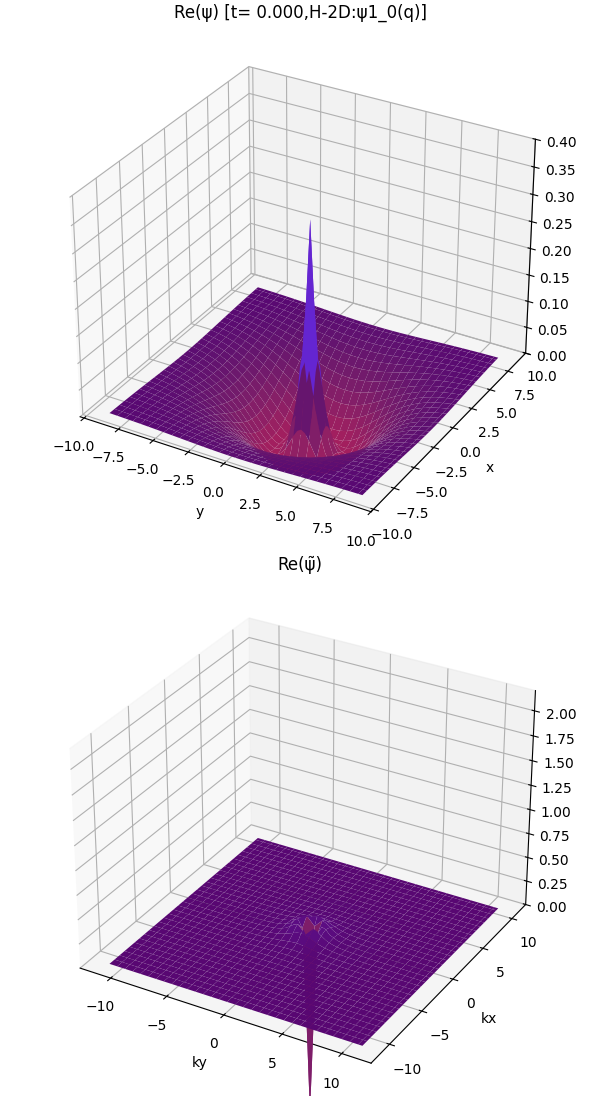
\includegraphics[width=1\columnwidth]{paper2025_figs/classic2D/6b_n1_m0/t_00.000_3d-qp.png}
        \caption{波動関数 $\PsiTwoD_{1,0}$}
        \label{subfig:initial-wavefunction-2d-1-0}
    \end{subfigure}
    \begin{flushleft}\small 

        (a) 主量子数$n=0$ 方位量子数 $m=0$ の基底状態 $\PsiTwoD_{0,0}$(式
        \ref{eq:psi2D00-wave-function})。 (b) $n=1,m=0$ の励起状態
        $\PsiTwoD_{1,0}$ (式\eqref{eq:psi2D10-wave-function})。それぞれ上段が
        real-spaceでの波動関数の実部の値で、下段はk-spaceでの実部の値。(a)と(b)
        は原点での波動関数の値が非ゼロである。

    \end{flushleft}
\end{figure}

\begin{figure}[ht]
    \centering
    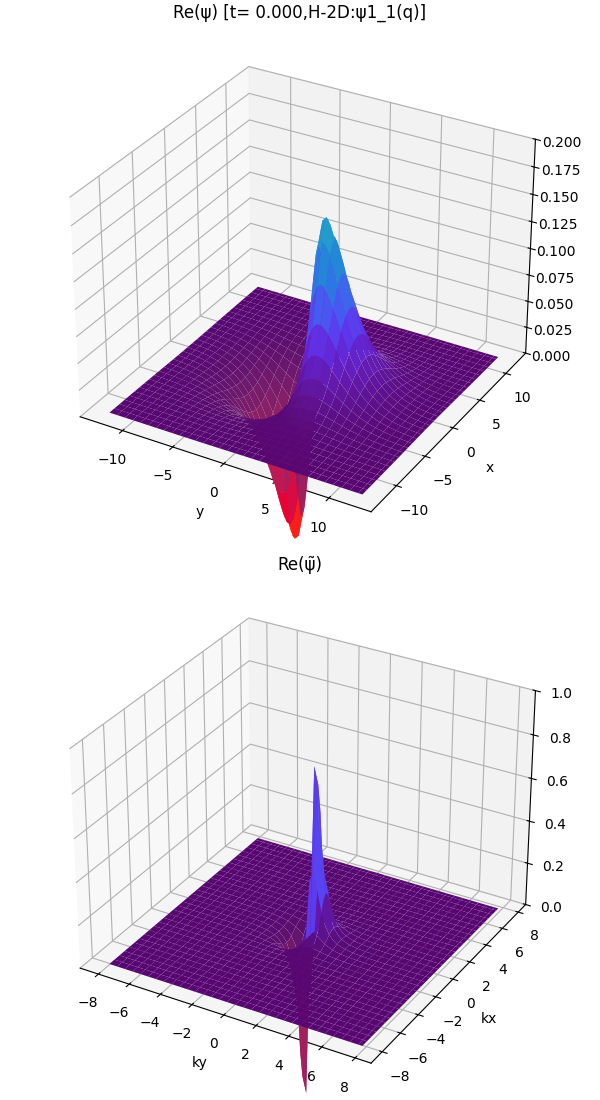
\includegraphics[width=0.45\columnwidth]{paper2025_figs/classic2D/6b_n1_m1/t_00.000_3d-qp.png}
    \caption{波動関数 $\PsiTwoD_{1,1}$}
    \label{subfig:initial-wavefunction-2d-1-1}
    \begin{flushleft}\small

        $n=1,m=1$ の励起状態 $\PsiTwoD_{1,1}$ (式
        \ref{eq:psi2D11-wave-function})。それぞれ上段がreal-spaceでの波動関数の
        実部の値で、下段はk-spaceでの実部の値。原点での波動関数の値がゼロであ
        る。

    \end{flushleft}
\end{figure}

\clearpage
\subsubsection{量子コンピュータエミュレータの使用}
本研究では量子回路を実行するのに量子コンピュータの実機ではなく、古典コンピュータ
上の量子コンピュータエミュレータを使用する。これは古典コンピュータ上で動くプログ
ラムであり、量子回路のSDKのツールの一つとして提供されている
\cite{website:qiskit-aer}。

量子コンピュータエミュレータはqubitの状態ベクトルの内容を古典コンピュータのメモ
リ上に保持し、qubitに対する演算については、重ねあわされた個々の状態に対する演算
に展開して実行する。

qubitの状態の表現方法にはいくつか方法があり、最も単純なstate vector法ではqubit数
$N$の状態ベクトルを、要素数$2^N$の配列としてメモリ上に保持する方法である。

qubitの量子もつれの程度が低く、遠く離れたqubit同士のもつれがほとんどない場合に
は、qubitを数珠繋ぎのような行列の連なりとして表現することでメモリ使用量を大幅に
圧縮する、Matrix Product State (MPS)法が知られており、Qiskitのエミュレータでも提
供されている\cite{Vidal2003.PhysRevLett.91.147902}。しかし、第一量子化における
qubitの使い方では、補助qubitを除いて全てのqubitを基本的にもつれさせるので、MPS法
によるデータ圧縮は望めない。そのため、本研究ではstate vector法を用いる。

また、エミュレータの機能として、量子コンピュータ実機のノイズモデルのシミュレー
ションがあるが、本研究のアルゴリズムは演算回数が多いため、ノイズが克服されたFTQC
での動作が前提となる。そのため回路設計としてノイズ影響下での動作を考慮していな
い。エミュレータを利用する際にはノイズをゼロとした理想的な量子コンピュータとして
動作させている。

\subsubsection{古典プログラムによる時間発展シミュレータの併用}
本研究のシミュレータ回路を量子コンピュータのエミュレータ上で動作させるには、回路
のqubit数とゲート数をエミュレータで扱える範囲に抑える必要がある。そのため、指定
できるモデルのパラメータの範囲は限られている。エミュレータで実行可能なパラメータ
の範囲を超える値について評価する時には、シミュレータ回路と等価な動作をするように
作成した古典プログラムを併用する。シミュレータ回路で実際に動作させたパラメータに
ついては第\ref{subsec:circuit-size-evaluation}節の表
\ref{tab:emulator-circuit-configurations}に示す。

\subsubsection{使用した計算環境}
シミュレーション計算に使用した計算機ハードウェアとソフトウェアは以下の通りである。
\begin{itemize}
    \item CPU:AMD Ryzen 9 7950X 16 Core × 1
    \item メモリ: 128GB
    \item GPU: NVIDIA GeForce RTX 4090 × 1
    \item OS: Ubuntu 22.04.4 LTS
    \item Quantum SDK: Qiskit 1.4.0, qiskit-aer-gpu 0.15.1
    \item 量子化学シミュレータソフトウェア: Chemical Reaction Simulator Q (crsQ) \cite{website:crsq}
\end{itemize}

\subsection{シミュレータ回路の構成の検討}

本節では、本研究の3つの検討内容の一つ目である、エミュレータで動作可能な回路構成
の検討について説明する。エミュレータに収まる回路構成とするために、計算回路の簡略
化と、計算モデルの簡略化の双方を検討する。計算回路の簡略化方法としては、クーロン
ポテンシャル回路の簡略化を検討する。計算モデルの簡略化については、モデルの次元数
を1と2に限定することと、原子核の位置を固定することを検討する。

量子化学シミュレーションの量子回路が必要とするqubit数やゲート数を見積もる一般的
なアプローチでは、計算を希望する分子モデルのサイズと許容する誤差から出発して、それ
に対応するために必要なqubit数とゲート数を見積もるが、本報告では逆に、利用可能な
qubit数から出発して、その上で動作可能な回路構成例を定める方法を検討する。そのた
めに、小規模モデルにおける具体的な規模数値に着目し、大規模モデルに対しては必ずし
も効率的ではない回路構成も取り上げる。

シミュレータ回路の回路規模の主要な部分がクーロンポテンシャルの計算回路である。
Suzuki-Trotter分解に基づく基本的なクーロンポテンシャルの計算回路では、シミュレー
ション対象の直方体空間を等間隔の格子に分割し、格子のインデクスを複数のqubitから
なるレジスタに対応させ、qubitの値に対する算術演算によりクーロンポテンシャルを計
算する\cite{Zalka-rspa.1998.0162}。算術演算には二進の演算回路を用いる
\cite{Vedral1996.PhysRevA.54.147}。このように構成された回路の規模は、粒子数の多
項式の量子ビット数とゲート数であり、古典計算機よりも指数的に効率がよい。これが基
本となる計算方法である。ただし、オーダーとしては効率的であるものの、必要な補助
qubitの数とゲート数の定数係数は決して小さくはない。

ゲート数を削減する工夫として、$1/\sqrt{x}$の近似値をQROMで求めた後に
$1/\sqrt{x}$を3次多項式で近似し、Newton-Raphson法で近似値の精度を高める方法が提
案されている\cite{Rubin2024.pnas.2317772121}。

本研究では新たに、ゲート数の増加は許容しても補助qubit数を削減する方法を検討する。

本節では上記の3つの方法について紹介し、1つ目と3つ目の方法については実際に回路と
して実装して評価する。

\subsubsection{算術演算ゲートによるポテンシャルの計算回路}
\label{subsec:potential-circuit-by-arithmetic-gates}

クーロンポテンシャル計算回路の基本となるのは算術演算回路に基づく方法である
\cite{Zalka-rspa.1998.0162}。

\begin{figure}[ht]
    \centering
    \begin{quantikz}[transparent]
        \lstick{$n_1$} & \qwbundle{\nb} & \gate[4]{\Thetaep} &                   & \gate[4]{\Thetaep} &\\
        \lstick{$n_2$} & \qwbundle{\nb} &                    &\gate[3]{\Thetaep} & \linethrough &\\
        \lstick{$n_3$} & \qwbundle{\nb} & \linethrough       &                   & & \\
        \lstick{$tmp$} & \qwbundle{} &                    &                   & &
    \end{quantikz}

    \caption{3電子系におけるクーロンポテンシャル項回路 $\Thetaep$ の例}
    \label{fig:theta-ep-multi-electron}
    \begin{flushleft}\small
        
        $n_1,n_2,n_3$はそれぞれ電子 1,2,3 の離散化された座標に対応するレジスタで
        あり、それぞれ$\nb$ビットからなる。qubitの線に付けられた斜線はその線が単
        一のqubitではなく複数のqubitからなるレジスタであることを示す。 $tmp$は補
        助qubitレジスタである。クーロンポテンシャル計算回路$\Thetaep$は3組の電子
        対 (1,2), (2,3), (1,3) のそれぞれに対して設ける必要があるが、補助qubitレ
        ジスタは1組だけでよい。$\Thetaep$回路の箱を貫通しているqubitの線はその回
        路がそのqubitを使用しないことを示す。
    \end{flushleft}
\end{figure}

この回路では計算途中の値を保持するための補助qubitを$O(\nb)$のオーダーで必要とす
るが、多数の粒子からなる系を扱う場合、粒子対の数の分だけ演算回路が必要となるもの
の、異なる粒子対に対する計算に対して一組の補助qubitを繰り返し使うことができる。
そのため、図\ref{fig:theta-ep-multi-electron}に示すように粒子数が増えても補助
qubitの数を一定に保つことができる。その結果、回路のqubit数の粒子数に対する依存性
の評価においては一般的に補助qubitの数自体は問題視されない。しかし、小規模モデル
においては補助qubitの個数が回路のqubit数の相当な割合を占める。

\clearpage
\subsubsection{QROMとNewton-Raphson法を併用するポテンシャルの計算回路}
\label{subsec:potential-circuit-by-qrom-newton-raphson}

第一量子化の時間発展シミュレーションの先行研究では、qubit数の定数因子については
受容している一方でゲート数については削減が模索されている。ゲート数の多い平方根と
除算を合わせて回避する改良案としてはQuantum Read Only Memory (QROM)で概算値を求
めてからNewton-Raphson法を1ステップ実行することで精度を高める方式が提案されてい
る\cite{Rubin2024.pnas.2317772121}。この方法では、$1/\sqrt{x}$を3次多項式で近似
し、 Newton-Raphson法を用いて解を求める。精度を高めるために、計算の定義域を区画
に分割して区画ごとに3次多項式の係数を変える。また、Newton-Raphson法を1ステップだ
けで済ませるために、$1/\sqrt{x}$の近似値をQROMで与える。QROMの元々の提案では、
QROM回路は入力ビットの指数のゲート数を必要とする
\cite{Babbush_2018b.PhysRevX.8.041015}。しかしここでは
\cite{Sanders2020.PRXQuantum.1.020312}で提案されたVariable Spacingという手法を用
いて、QROM回路のゲート数をビット数のオーダーまで抑えている。

この方法では平方根と除算の回路を回避できるため、ゲート数を削減することができる
が、 QROM回路が必要とする補助qubit数は多い。QROM回路は出力ビット数に比例した補助
qubit数を必要とするためである。小規模モデルにおいては補助qubit数が回路全体の
qubit数に占める割合が大きくなる。利用可能なqubit数が多い量子コンピュータ上で粒子
数がある程度多い大規模モデルを扱う場合に有効な方法である。

この方式は必要とするqubit数が多く、エミュレータによる動作が困難であるため、本研
究においてはこの方法の実装はしていない。

\subsubsection{UCRZゲートによるポテンシャルの計算回路}
\label{subsec:potential-circuit-by-ucrz-qubits}

本研究では、定数個の補助qubit数も問題視し、これを削減する手段としてQROMと作用が
似ている回路であるUniformly Controlled Rotation (UCR)回路に着目する
\cite{Mottonen2004.PhysRevLett.93.130502}。UCR回路のバリエーションのひとつ、UCRZ
回路では回路の出力がターゲットとするqubitの位相回転角として得られる。これはクー
ロンポテンシャル回路の出力と形式が同じであるので、UCRZ回路の出力をクーロンポテン
シャル回路の出力としてそのまま使うことができる。UCRZ回路が必要とする補助qubit
は、ターゲットqubit一つだけであるので、算術演算回路に比べて補助qubitを大幅に減ら
すことができる。ただし、この回路のゲート数はQROM回路と同様にコントロールレジスタ
の指数となるので、大規模なモデルへの適用は現実的ではない。小さいモデルにおいて有
効な選択肢である。UCRZ回路は総qubit数が限定されている場合の代替の回路として有用
である。本研究ではUCRZ回路を用いることによって2次元モデルの計算がエミュレータ上
で実行可能な回路構成を実装して評価する。

UCR回路は$n$ビットの入力レジスタの値のビット列に応じて単一のターゲットqubit $t$
に特定の回転軸$a$ まわりの回転を与える回路である
\cite{Mottonen2004.PhysRevLett.93.130502}。入力値に対して事前に指定された値を出
力するという点で、UCR回路の働きはQROM回路の一種とみなすことができる。一般のQROM
が出力を出力レジスタ上のビット列として出力するのに対してUCR回路はターゲットqubit
の回転角として出力する。UCRZ回路は出力がターゲットqubitの位相変化であるため、時
間発展演算子のポテンシャル項の計算にそのまま使うことができ、粒子間の距離計算と逆
数計算とを単一のUCRZ回路で置き換えることができる。その結果算術演算回路で必要な多
数の補助qubitを省略することが可能になる。

UCR回路の作用を式で表すと
\begin{equation}
    \ket{b}\ket{t} \mapsto \ket{b} R_{\mathrm{a}}(\theta_{\mathrm{b}})\ket{t}
\end{equation}
となる。

\begin{figure}[ht]
    \centering
    \begin{quantikz}[column sep=0.3cm]
        \lstick{$b_0$} & & \ctrl{3} & &          & & \ctrl{3} & &          & & \ctrl{3} & &          & & \ctrl{3} & &          &\\
        \lstick{$b_1$} & &          & & \ctrl{2} & &          & &          & &          & & \ctrl{2} & &          & &          &\\
        \lstick{$b_2$} & &          & &          & &          & & \ctrl{1} & &          & &          & &          & & \ctrl{1} &\\
        \lstick{$t$} & \gate{\mathrm{R_0}} & \targ{} & \gate{\mathrm{R_1}} & \targ{} & \gate{\mathrm{R_2}} & \targ{} & \gate{\mathrm{R_3}} & \targ{} &
                       \gate{\mathrm{R_4}} & \targ{} & \gate{\mathrm{R_5}} & \targ{} & \gate{\mathrm{R_6}} & \targ{} & \gate{\mathrm{R_7}} & \targ{} &
    \end{quantikz}
    \caption{3ビット入力のUCRZ回路の例}
    \label{fig:ucrz-n3}
    \begin{flushleft}\small 3ビットの入力レジスタ$b_2b_1b_0$に対して8通りの入力
    値があり、それぞれに対応する8個のRzゲートがターゲットqubitに対して作用す
    る。$\mathrm{R}_k$は$\mathrm{Rz}(\theta_k)$を表す。 各Rzゲートは事前に指定
    された回転角$\theta_k$で位相を回転させる。Rzゲートの前後にC-NOTゲートが配置
    されており、入力レジスタのビット列に応じてRzゲートの作用が反転する。
    \end{flushleft}
\end{figure}

$n$ビット入力のUCRZ回路は、ターゲットqubitに対するC-NOTとRzゲートを交互に$2^n$個
並べた回路である。3ビット入力のUCRZ回路の例を図\ref{fig:ucrz-n3}に示す
\cite{Mottonen2004.PhysRevLett.93.130502}。

$k$番目のRzゲート$\mathrm{R}_k$は事前に決めた角度$\theta_k$
だけ位相を回転させる。全てのC-NOTが反転しない場合、回路全体での回転角は
$\theta_k$ の合計値になる。しかし、反転するC-NOTが存在する場合、反転するC-NOTに挟
まれる全てのRzゲートは$\mathrm{XR_z}(\theta)\mathrm{X}=\mathrm{R_z}(-\theta)$の関係から、回転角の符号が反転する。行列
で表すと
\begin{equation}
    \mathrm{XRz}(\theta)\mathrm{X} = \begin{pmatrix}
        0 & 1 \\
        1 & 0
    \end{pmatrix}
    \begin{pmatrix}
        e^{-i\theta/2} & 0 \\
        0 & e^{i\theta/2}
    \end{pmatrix}
    \begin{pmatrix}
        0 & 1 \\
        1 & 0
    \end{pmatrix}
    = \begin{pmatrix}
        e^{i\theta/2} & 0 \\
        0 & e^{-i\theta/2}
    \end{pmatrix}
    = \mathrm{Rz}(-\theta)
\end{equation}
である。

C-NOTのコントロールビットには入力レジスタ $b$のいずれかのビットがつながれるの
で、 $b$ の値に応じて作用が反転するRzゲートが変わる。その結果、入力 $b$ に対して
出力される回転角の合計値 $\alpha_b$ は$\alpha_b=\sum_{k}{(-1)^{f_k(b)}\theta_k}$
のようになる。すなわち、$\theta_k$ の符号を $k,b$ に応じて決めて加算した値とな
る。$\theta_k$から$\alpha_b$ への写像は逆写像が知られているので、各bに対して所望
の $\alpha_b$ が得られるように$\theta_k$ を定めることができる。

クーロンポテンシャル項回路においては、粒子の座標のqubitをUCR回路の入力qubitの$b$を
通し番号とする格子点$\bm{\chi}_b$に対応させ、その格子点でのポテンシャルエネルギー
$\Hp(\bm{\chi}_b)$に基づいてターゲットqubitの位相回転角$\alpha_b$を
\begin{equation}
\alpha_b = -\frac{\Hp(\bm{\chi}_b)\deltat}{\hbar}
\end{equation}
と指定することで、求める時間発展演算子のポテンシャルエネルギー項回路となる。

\subsection{クーロンポテンシャルの極の扱い}
\label{sec:coulomb-potential-handling}

本研究では原子モデルを扱うためクーロンポテンシャルを量子回路によって計算する。
クーロンポテンシャルの計算においては、極の扱い方を定める必要がある。時間発展計算
においてはポテンシャル$-1/r$と波動関数$\psi$の積が各格子点の座標で計算される。こ
の積をポテンシャルの極で計算すると発散してしまう。これに対処する方法は大きく2つ
に分類される。(a)粒子間距離が０でも発散を起こさないようなポテンシャルの近似式を
導入する方法と、(b)原子核と電子の座標の離散化の定義を変えることで計算上では両者
の距離がゼロになることを防ぐ方法である。 (a)の近似式の例を2つ検討する。一つ目の
近似式(a1)は、局所平均(local average)ポテンシャルと著者らが呼ぶ近似式で、極での
ポテンシャルの値として極近傍の領域での平均値を用いる方法である。二つ目の近似式
(a2)は、soft coreポテンシャルとして知られている方法で、粒子間距離を求めるノルム
計算にオフセット項を加えたポテンシャル関数である。この関数はハミルトニアンシミュ
レーションにおいてクーロン項計算の発散を防ぐ手段としても検討されている
\cite{Childs2022quantumsimulationof,Kivlichan_2017}。また、電子の運動方向が拘束
されている物理系のモデルとしても分析されている\cite{Hall2009.PhysRevA.80.032507,
Fernandez_1991, LiChen2021.doi:10.1021/acs.jpca.1c00698}。

(b)の原子核と電子の座標の離散化の定義を変える方法の例としては、
電子の位置は格子の中心になるものと定義しておく一方で、原子核の座標はここから格子
の刻みの1/2だけいずれかの軸方向にずらした位置として定義する方法が提案されている
\cite{Chan2023.sciadv.abo7484}。この方法ではポテンシャルの極の近傍でTrotter誤差
が大きくなるため、Chanらは計算結果を後付けの演算処理で補正している。本研究では
(b)の手法は取り上げない。

時間発展演算子のポテンシャルエネルギー項の回路 $\Thetaep$ ではクーロンポテンシャ
ルと波動関数の値の積が計算される。クーロンポテンシャルの分母のゼロが実際に問題と
なるのは、波動関数の値がポテンシャルの極においてゼロではない場合であり、本報告で
扱う波動関数の中でこれに該当するのは、2次元モデルの波動関数のうち方位量子数$m=0$
である$\Psi_{0,0}^{\mathrm{2D}}$と$\Psi_{1,0}^{\mathrm{2D}}$ の二つである。以下
ではこれら二つの固有解に着目する。

\subsubsection{局所平均ポテンシャルを用いる方法}
(a1)の近似式(local average ポテンシャル)は、極の座標以外では本来の式を用い、極においては
粒子間距離 $r=0$の代わりに実効半径 $\reff$を用いる式として次のように定義する。
\begin{equation}
\Hla(r) = \begin{cases}
-\frac{1}{r} & (r>0) \\
-\frac{1}{\reff} & (r=0)
\end{cases}\label{eq:Halr}
\end{equation}
$\Hla$は、回路としての実装コストを抑えることができる式である。
$r=0$の時に除算の分母を置き換える回路により実現できる。

まず、$\Hla$において $\reff$ を選ぶ方法について述べる。ここでは波動関数が既
知である場合の式の導出を示す。

1次元モデルの $\PsiOneD_1$ においてはポテンシャルの極での波動関数の値がゼロであ
り、ポテンシャルの値は有限であればよい。

2次元モデルにおいては、方位量子数$m$の値に応じて、ポテンシャルの極における波動関
数の値がゼロである場合と非ゼロである場合とがある。$m\ne0$の解ではゼロにな
り、$m=0$では非ゼロになる。非ゼロの関数の例として$\PsiTwoD_{0,0}$ と
$\PsiTwoD_{1,0}$を取り上げて、$r=0$におけるポテンシャル関数の適切な値を検討す
る。$m=0$の場合は代表値は任意の値でよいので、$m=1$の場合に対して求めた$\reff$
の値を、$m=0$の場合にも適用することができる。

近似式 $\Hla$ におけるパラメータ $\reff$ は、次のように定めることができる。
クーロンポテンシャル項の計算では、各グリッドの中心座標におけるポテンシャルの値を
代表値として用いて、それにグリッドの面積を掛けることで積分値を近似する。極と重な
る格子点ではこの代表値が発散してしまうが、格子の領域内で積の平均値を求める積分計
算は２次元以上のモデルであれば発散しない。そこで、積分値と同じ値が得られるような
代表値でもって、極におけるポテンシャルの近似値に定めることを考える。

極を中心としたグリッドの内接円を考え、その円内のクーロンポテンシャルの代表値が
$-1/\reff$ であるとした時のエネルギーの値 $W_{n,m}^\prime$ を計算する。次に、
同じ領域に対して真のクーロンポテンシャルを用いて計算したエネルギーの値 $W_{n,m}$
を計算する。その後、両者が一致するように $\reff$ の値を求める。これを
$(n,m)=(0,0)$と$(1,0)$ のそれぞれに対して求める。$W_{n,m}$と$W_{n,m}^\prime$はそ
れぞれ、
\begin{align}
    W_{n,m}&=\int_{\theta=0}^{2\pi}d\theta\int_{r=0}^{\deltar/2}
    \Hep(r)\abs{\PsiTwoD_{n,m}(r)}^2r dr\\
    W_{n,m}^\prime&=\pi\left(\frac{\deltar}{2}\right)^2
    \Hla(0)\PsiTwoD_{n,m}(0) \notag \\
    &=-\frac{\pi\deltar^2}{4\reffnm{n,m}}
    \sqrt{\frac{q_0^3(n-\abs{m})!}{\pi(n+\abs{m})!}}
    L_{n-\abs{m}}^{2\abs{m}}(0)
\end{align}
である。$(n,m)=(0,0)$と$(1,0)$に対してそれぞれ$W_{n,m}=W_{n,m}^\prime$ を解くと、
\begin{align}
    \reffnm{0,0} &=\frac{q_0\deltar^2}{4(-e^{-q_0\deltar}+1)}
    \simeq \frac{q_0\deltar^2}{4(-1+q_0\deltar+1)}=\frac{\deltar}{4}
    \label{eq:delta-1-0-0}\\
    \reffnm{1,0} &=\frac{q_0\deltar^2}{4((-1+q_0^2\deltar^2)e^{-q_0\deltar}+1)}
    \simeq \frac{q_0\deltar^2}{4((-1+q_0^2\deltar^2)(1-q_0\deltar)+1)}
    \simeq\frac{\deltar}{4}
    \label{eq:delta-1-1-0}
\end{align}
が得られる。近似はいずれも$\deltar\ll1$ である場合のものである。導出は付録
\ref{chap:appendix_derivation_derivation}に示す。

これらの式を用いて時間発展をさせた時に得られるエネルギー値の評価を
\ref{subsubsec:results-local-average-potential}項で示す。

\subsubsection{soft core ポテンシャルによる近似式}
(a2)の近似式は、距離を求めるノルム計算にオフセット項を加えた、soft core
ポテンシャルの式であり、次のように定義する\cite{Kivlichan_2017}。
\begin{equation}
\Hsc(r) = -\frac{1}{\sqrt{r^2+\Delta^2}}
\label{eq:Hsc2r}
\end{equation}

分母がゼロになることを防ぐ目的で導入される定数$\Delta$の定め方には二通りの
アプローチがある。一つ目のアプローチは、次元数を1ないし2に下げた数値計算モデルに
おいて、得られるエネルギーの計算結果を3次元のモデルの計算結果に近づけるように
定める方法である。この方法においては、1次元の水素原子モデルの計算において
$\Delta=\sqrt{2}$と定めることで、エネルギー固有値として3次元の水素原子
と同じ$-0.5$が得られることが知られている\cite{Eberly1991.PhysRevA.44.5997}。
このアプローチに従う場合、$\Delta$を導入する目的は特異点の正規化ではなく、
エネルギー値の補正であるため、その観点では補正の必要のない三次元のモデルに
おいては$\Delta=0$となり、特異点は温存されることになる。

二つ目のアプローチは、特異点の正則化を動機として$\Delta$を定める方法である。
このアプローチに沿った$\Delta$の選択に関して具体的に論じられている例は見られない。

soft coreポテンシャルは、$r=0$の点においては、soft core ポテンシャルの式
\ref{eq:Hsc2r}と局所平均ポテンシャルの式\ref{eq:Halr}は同様に定数値となる。この
点に着目し、本研究では極において両者が一致するように$\Delta$を定めて数値評価す
る。
この値を用いて時間発展をさせた時に得られるエネルギー値の評価を
\ref{subsubsec:results-local-average-potential}項で示す。


\subsection{誤差を最小にするシミュレーションパラメタの決定}
\label{sec:parameter-selection-for-minimum-error}

ハミルトニアンシミュレーションを行うにはいくつかのシミュレーションパラメータの設
定が必要になる。計算誤差を所望の範囲に収めるために必要となるシミュレーションの空
間分解能やステップ時間の検討は多くされており、所望の精度を得るために必要となる
qubit数の算出が検討されている\cite{FEIT1982412, Kivlichan_2017,
Chan2023.sciadv.abo7484}。 本報告では既存の検討とは逆に、qubit数が所与の場合にシ
ミュレーションパラメータに課される制約条件やトレードオフ関係に着目して最良な精度
をもたらすパラメータの決定方法を示す方法を検討する。本報告では時間発展にTrotter
分解を用いるが、グリッド法で定義されたモデルにTrotter分解で時間発展させた場合に
計算結果として得られる波動関数には、以下の誤差が含まれる。

\begin{equation}
\errtotal \leq \errspatial + \errtemporal
\label{eq:error-total-decomposition}
\end{equation}

ここで $\errtotal$ は誤差の合計、$\errspatial$ は空間離散化のパラメータに起因す
る誤差、$\errtemporal$ は時間離散化のパラメータに起因する誤差である。両者はさら
に要素に分解される。それぞれの要素ごとに特性が知られているが、特定の要素だけ改善
しても他の要素の成分が優勢の場合には全体としての改善が得られない。そこで、トレー
ドオフ関係を考慮しながら支配的な誤差項を削減していくことが必要になる。

トレードオフとして本報告で考察するのは空間座標の刻み$\deltar$と、シミュレーショ
ン対象直方体の１辺の長さ$L$の関係である。グリッド法では計算対象の直方体空間を定
めてその領域に収まる範囲の波動関数を計算する。領域外では波動関数の振幅が無視され
るので、得たい精度に照らして領域の境界での波動関数の振幅が無視できる大きさとなる
ように十分大きな寸法に設定することが必要である。領域の一辺の長さ$L$が所望の精度
に照らして十分であるかどうか判断する方法として、シミュレーション対象の波動関数か
ら領域境界面上の電子密度の最大値を数値的に算出し、それが目標値$\rho_0$以下となる
ように$L$を定める方法が提案されている\cite[Supplementary material, S8, A. Space
Cost]{Chan2023.sciadv.abo7484}。$L$を拡大するにはqubitの数を増やすか、分解能を粗
くする必要がある。qubit数が多い計算環境下では必要に応じてqubit数を増やすことがで
きるが、qubit数が制限されている条件下では座標の量子化の刻み$\deltar$を大きくする
ほかない。この場合、空間の寸法と分解能がトレードオフ関係になる。このトレードオフ
を加味した寸法の決定方法については今まで具体的に論じられていない。本報告では波動
関数を仮定した上でこのトレードオフを数値的に評価し、適切なパラメータの値を決定す
る方法を示す。

時間刻み$\deltat$の満たすべき条件は２つあり、離散的フーリエ変換を用いることでサ
ンプリング定理からの要請に基づく条件\cite{FEIT1982412}とTrotter分解の誤差に起因
する条件である
\cite{Childs2021.PhysRevX.11.011020,Burgarth2024.PhysRevResearch.6.043155}。これ
らの両方を考慮する必要がある。

誤差を空間パラメータによる誤差と時間パラメータによる誤差に分かれると示した式
\ref{eq:error-total-decomposition}はさらに以下の要素に分けられる。
\begin{align}
    \errspatial &\equiv \errdisc + \errcutoff \\
    \errtemporal &\equiv \erralias + \errtrotter
\end{align}
ここで、$\errdisc$ は空間離散化による波動関数の近似誤差であり、$\errcutoff$ は計
算対象領域の直方体からはみ出た部分の波動関数の成分による誤差である。ま
た、$\erralias$ は有限の項数で波数表示されていることに伴うエイリアシング誤差であ
り、$\errtrotter$ はTrotter近似に起因する誤差である。

本節ではqubitの総数が所与の条件でこれらの誤差を小さくしていくためのパラメータの
決定方法を示す。空間パラメータによる２つの誤差 $\errdisc$ と $\errcutoff$ の対は
トレードオフ関係にあるので、トレードオフを考慮したパラメータ値 $\deltar$ の決定
方法を検討する。時間パラメータ $\deltat$ に関してはトレードオフが存在せず、サン
プリング定理から$\deltat$の上限値が、Trotter誤差の解析的評価からは予想される誤
差の上限が与えられるので、これらを考慮してパラメータを決定する。

\subsubsection{格子間隔の決定方法}
\label{subsec:delta-r-selection-method}
本報告ではシミュレーション対象領域は周期境界条件を適用しており、空間の一辺の長さ
は格子間隔$\deltar$を用いて各次元で共通で$L=2^{\nb}\deltar$ と表される。この空間
の中央を座標系の原点とし、原点に原子核を配置する。座標値が $[-L/2,L/2]$ からはみ
出る部分に関しては波動関数がカットオフされることになる。$\deltar$を小さくとる
と、$\errdisc$ が小さくなるという点では好ましいが、$\deltar$に比例して$L$も小さ
くなるため、$\errcutoff$ は増大してしまう。計算対象領域内の$\errdisc$
と、$\errcutoff$ が拮抗する $\deltar$ を探すことで、二種類の誤差の合計を最小にす
る $\deltar$ を求めることができる。

波動関数の二乗をシミュレーション領域上で積分した値$S_1$と領域外で積分した値$S_2$
をそれぞれ
\begin{align}
S_1 &= \int_{x,y,z=-L/2}^{L/2}\Psi(\bm{r})^{\ast}\Psi(\bm{r}) d\bm{r} \\
S_2 &= 1 - S_1
\end{align}
とする。

$S_1$に相当する離散化した座標での近似値を$S_d$とする:
\begin{equation}
S_d = \sum_{j}\abs{\Psi(\chij)}^2 \deltar^3
\end{equation}
このようにとると、
\begin{align}
\errdisc &\simeq \abs{S_1 - S_d} \label{eq:err-disc-definition}\\
\errcutoff &\simeq S_2 \label{eq:err-cutoff-definition}
\end{align}
となる。$\abs{S_d-S_1}+S_2$が最小となる$\deltar$が最適な$\deltar$の値である。

座標のqubit数 $\nb$ が一定の条件下で空間離散化のパラメータ $\deltar$ を変化さ
せるとグリッド数 $2^{(\nb)}$ は一定であるので $L=2^{(\nb)} \deltar$ が同時に増減
する。$\deltar$ が大きいと離散化誤差 $\errdisc$ が増大し $L$ が小さいとカット
オフ誤差 $\errcutoff$ が増大する。2つの誤差のトレードオフを考慮して $\deltar$ を
定める必要がある。

一次元のモデル $\psi_1^{1D}$ においていくつかの $\nb$ の値に関して離散化誤差
$\errdisc=|S_d-S_1|$ とカットオフ誤差 $\errcutoff=S_2$ を比較したグラフを
図 \ref{subfig:dq-tradeoff-1d} に示す。

グリッドの点が最も少ない $\nb=6$ の場合に着目すると、(A1)により、$S_2$の線と
$|S_d-S_1|$の線は$\deltar=0.22$ のあたりで交差する。(A2)においては$\nb=6$の線が
最小になる点に該当する。この値が2種類の誤差のトレードオフがバランスする値
である。$\deltar$と$L$ は比例しており(A3)からこの時 $L=14$ である。

qubit数が2つ多い $\nb=8$のケースに着目すると(A2)から、$\deltar=0.07\sim0.14$ の
範囲で値はほぼ0となっている。これは、この範囲で$\deltar$を変化させても、誤差の目
立った増減はないことを意味する。$\deltar<0.07$で値が急減するのは、$L$ が小さく
なってカットオフによる誤差が顕在化するためである。$\deltar>0.14$ で値が増加して
いくのは離散化誤差が顕在化するためである。qubit数が多い程、(A2)の値がほぼ最小とな
る $\deltar$ の範囲が広くなり、$\deltar$を自由に選べるようになる。

２次元モデルの波動関数 $\Psi_{0,0}^{2D}$ と $\Psi_{1,0}^{2D}$ に対するグラフを
図\ref{subfig:dq-tradeoff-2d-0-0} と \ref{subfig:dq-tradeoff-2d-1-0}にそれぞれ示
す。波動関数の広がりの違いに応じて適切な $\deltar$ の範囲が大きく変わることが分
かる。

\begin{figure}[ht]
    \centering
    \begin{subfigure}{1.0\columnwidth}
        \centering
        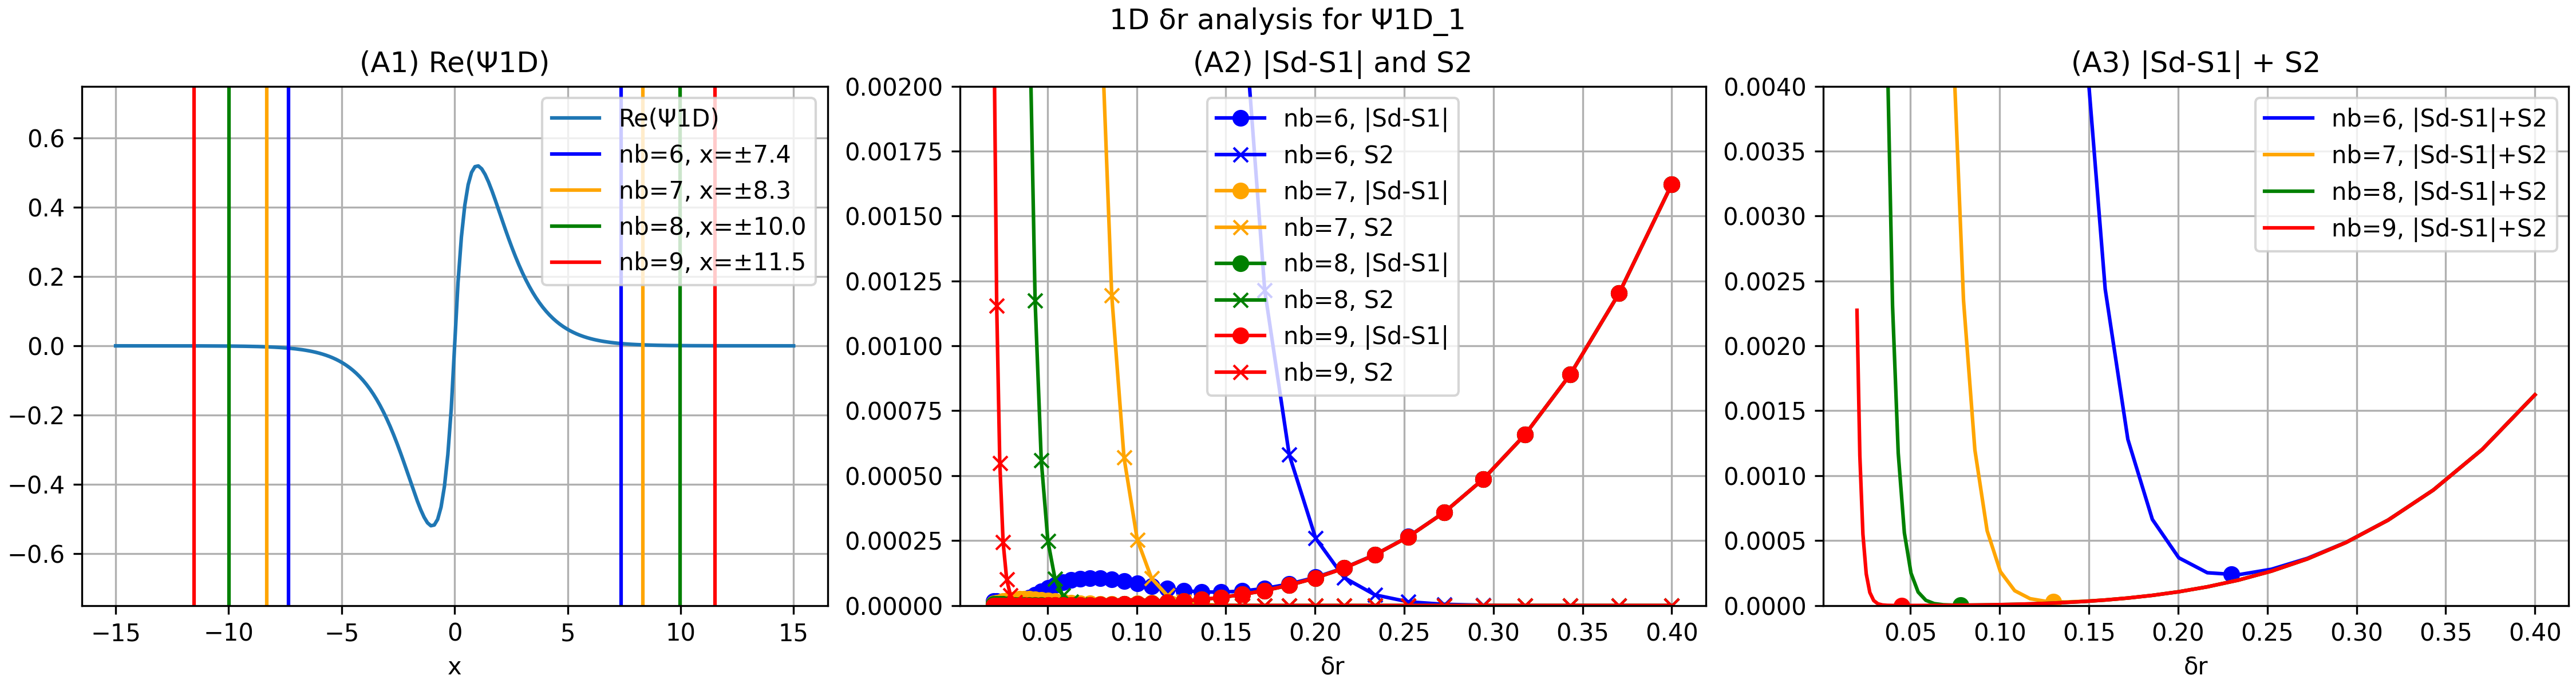
\includegraphics[width=\columnwidth]{paper2025_figs/dq_tradeoff/eval1d_dq.png}
        \caption{1次元モデル $\PsiOneD_1$}
        \label{subfig:dq-tradeoff-1d}
    \end{subfigure}
    \begin{subfigure}{1.0\columnwidth}
        \centering
        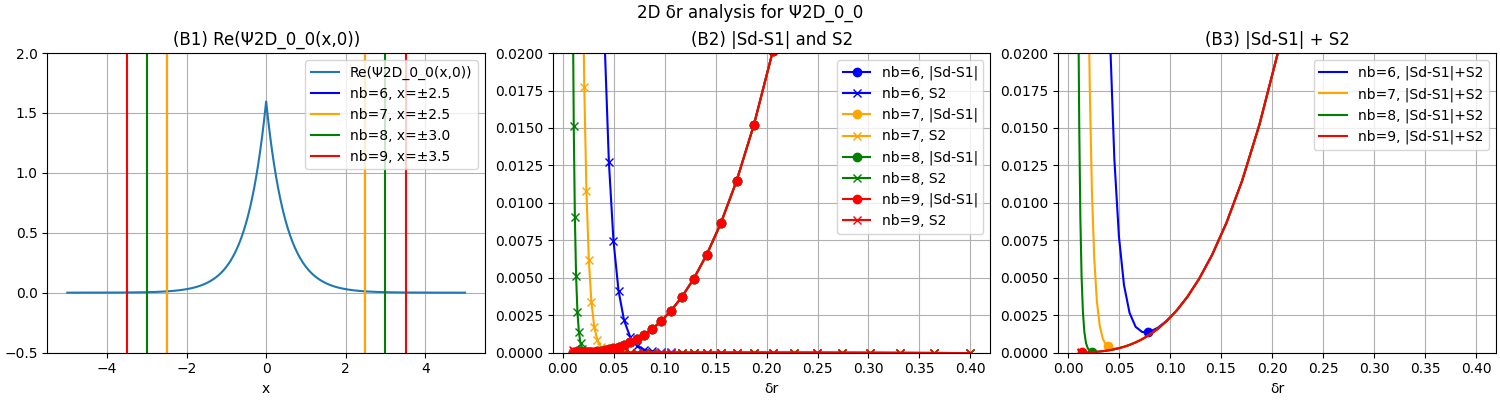
\includegraphics[width=\columnwidth]{paper2025_figs/dq_tradeoff/eval2d_dq_geom_0_0.png}
        \caption{2次元モデル $\PsiTwoD_{0,0}$}
        \label{subfig:dq-tradeoff-2d-0-0}
    \end{subfigure}
    \begin{subfigure}{1.0\columnwidth}
        \centering
        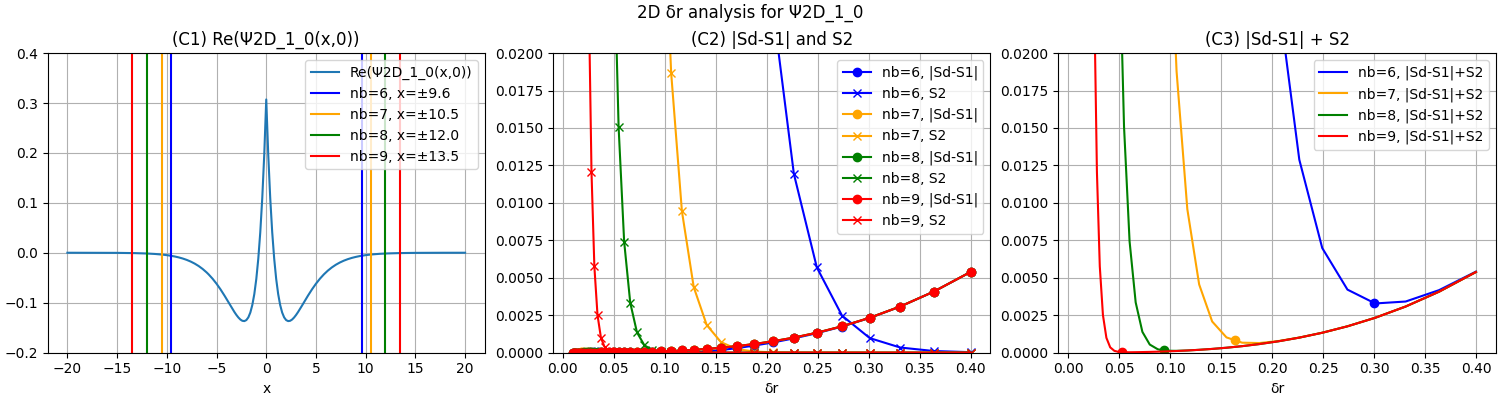
\includegraphics[width=\columnwidth]{paper2025_figs/dq_tradeoff/eval2d_dq_geom_1_0.png}
        \caption{2次元モデル $\PsiTwoD_{1,0}$}
        \label{subfig:dq-tradeoff-2d-1-0}
    \end{subfigure}
    \caption{いくつかの $\nb$ における$|\Sd-S_1|$と$S_2$の関係}
    \label{fig:dq-tradeoff}
    \begin{flushleft}\small

        (a)は1次元の $\PsiOneD_1$ に関するグラフ。(b), (c)はそれぞれ二次元の
        $\PsiTwoD_{0,0},\PsiTwoD_{1,0}$ に関するグラフ。(A1)から(C1)は波動関数
        の$y=0$切片における実部の値を示しており、選ばれた$\deltar$に対する
        $\pm L/2$の位置が垂直線で示されている。(A2)から(C2)は        
        $|\Sd-S_1|$と
        $S_2$を別の線としてプロットしており(式\eqref{eq:err-disc-definition},
        \ref{eq:err-cutoff-definition})、(A3)から(C3)が両者の和をプロットしてい
        る。誤差の和が最小となる点がトレードオフが均衡する点であり、最適な
        $\deltar$の値である。

    \end{flushleft}
\end{figure}
\clearpage

\subsubsection{サンプリング定理に基づく時間刻みの条件}

\label{subsubsec:deltat-selection-by-sampling-theorem}
時間刻み$\deltat$を定める根拠としては、サンプリング定理に由来する条件と、Trotter
分解の誤差に由来した条件がある。まず、サンプリング定理に基づく条件について検討す
る。

Trotter分解による時間発展によって求まる波動関数の各ステップでの値をサンプリング
された信号ととらえると、サンプリング定理により信号の中の最も高い周波数成分の２倍
のサンプリング周波数、すなわち $1/\deltat$ よりも高い周波数を用いる必要があ
る。Suzuki-Trotter分解の計算の文脈ではポテンシャルエネルギー項と運動エネルギー項
のそれぞれにおいて、時間発展の１ステップでの位相の変化量が半周期分、すなわち$\pi$
以下であることを意味する。
\begin{align}
\max_{\bm{r}}\abs{\Hep(\bm{r})\deltat/\hbar} < \pi \label{eq:nyqist-limit-by-hep}\\
\max_{\bm{k}}\abs{\Hek(\bm{k})\deltat/\hbar} < \pi \label{eq:nyqist-limit-by-hek}
\end{align}
それぞれの式は、波動関数が所与の条件下では以下のように具体的に求めることができる。

まず、本報告の１次元モデルの場合について検討する。位置エネルギー項に関する不等式
\ref{eq:nyqist-limit-by-hep}を解こうとした場合、そのままでは極において$\Hep$が
発散してしまう。時間発展計算においては、発散を起こさないように$\Hep$に近似を導入す
るので、その近似式を用いて評価する。

クーロンポテンシャルの極の扱いの節で述べたように1次元モデルにおけるハミルトニア
ンの近似式は$\Hla(r)$で$\reff=\deltar/2$ と置いたものである。格子点座標につ
いて記述すると
\begin{equation}
\HlaOneD(\chij) = \begin{cases}
-\frac{1}{\abs{\chij}} & (\chij\neq0) \\
-\frac{2}{\deltar} & (\chij=0)
\end{cases}
\end{equation}
である。$\abs{\HlaOneD}$が最大となるのは $\chij=0$ の時であり、
\begin{equation}
\max_{j}\abs{\Hep(\chij)} = \frac{2\deltat}{\deltar\hbar}<\pi
\end{equation}
となる。これを$\deltat$について解くと、
\begin{equation}
\deltat < \frac{\pi\deltar\hbar}{2}=\frac{L\pi\hbar}{2^{\nb+1}}\equiv\deltatPmaxOneD
 \label{eq:nyqist-limit-by-hep-final}
\end{equation}
を得る。ここで、$\deltar=L/2^{\nb}$を用いた。

同様に、運動エネルギー項に関する不等式\eqref{eq:nyqist-limit-by-hek}からは、
\begin{equation}
\max_{\ell}\abs{\frac{\hbar^2(\kellx)^2}{2}\times\frac{\deltat}{\hbar}} < \pi
\label{eq:nyqist-limit-by-hek-maximum}
\end{equation}
が得られる。波数$\kaplx$の絶対値が最大となるのは波数のインデクス
$\ell=\kaplx=-2^{\nb-1}$の時でありその時の
$\kellx=\kaplx\deltak=(-2^{\nb-1})\times2\pi/L$となる。これを用いると式\eqref{eq:nyqist-limit-by-hek-maximum}は、
\begin{equation}
    \frac{\hbar^2}{2}\left(\frac{2\pi}{L}\times 2^{(\nb-1)}\right)^2\times\frac{\deltat}{\hbar} < \pi
\end{equation}
となり、これを$\deltat$について解くと
\begin{equation}
\deltat < \frac{L^2}{2^{2\nb-1}\hbar\pi}\equiv\deltatKmaxOneD
 \label{eq:nyqist-limit-by-hek-final}
\end{equation}
となる。時間発展の期間$T$とTrotter分割数 $\nT$を用いると $\deltat=T/\nT$ となること
から、$\deltat$に関するこれらの上限値に対応する分割数の下限値をそれぞれ
\begin{align}
    \nTpminOneD &= \frac{T}{\deltatPmaxOneD}=\frac{2^{\nb+1}T}{L\pi\hbar}
    \label{eq:nT-pmin-definition}\\
    \nTkminOneD &= \frac{T}{\deltatKmaxOneD}=\frac{2^{2\nb-1}\pi\hbar T}{L^2}
    \label{eq:nT-kmin-definition}
\end{align}
と定める。時間発展の分割数$\nT$はこれらのいずれよりも大きい値にする必要がある。

次に２次元モデルについて同様に検討する。

まず位置エネルギー項に基づく不等式\eqref{eq:nyqist-limit-by-hep}については、2次元
モデルにおいても1次元モデルと同様に極における発散を防ぐために $\Hep$ には近似式
を用いる。次節で検討するように２つの近似式 $\Hla$,\ $\Hsc$ のパラメータは共に
$\reff=\Delta=\deltar/4$ を用いる。格子点座標に基づいて書くと
\begin{align}
\HlaTwoD(\chij) &= \begin{cases}
    -\frac{1}{\abs{\chij}} & (\chij\neq0) \\
    -\frac{4}{\deltar} & (\chij=0)
\end{cases}\\
\HscTwoD(\chij) &= -\frac{1}{\sqrt{\abs{\chij}^2+(\deltar/4)^2}}
\end{align}
これらを用いると式\eqref{eq:nyqist-limit-by-hep} の最大値は等しく
\begin{equation}
\max_{j}\abs{\HlaTwoD(\chij)\deltat/\hbar}
  = \max_{j}\abs{\HscTwoD(\chij)\deltat/\hbar}
  = \frac{4\deltat}{\deltar\hbar} < \pi
\end{equation}
となり、これより
\begin{equation}
\deltat < \frac{\pi\deltar\hbar}{4}
        =\frac{L\pi\hbar}{2^{\nb+2}}
        \equiv\deltatPmaxTwoD
 \label{eq:nyqist-limit-by-hep-final-2D}
\end{equation}
を得る。

運動エネルギー項に基づく不等式\eqref{eq:nyqist-limit-by-hek}からは、
\begin{equation}
\max_{\ell}\abs{\frac{\hbar^2((\kellx)^2+(\kelly)^2)}{2}\times\frac{\deltat}{\hbar}} < \pi
\label{eq:nyqist-limit-by-hek-maximum-2D}
\end{equation}
波数$\kellx,\kelly$ の二乗和が最大となるのは $\kaplx=\kaply=-2^{\nb-1}$の時であ
り、その時の $\kellx=\kelly=\kaplx\deltak=\kaply\deltak=-2^{\nb-1}\times2\pi/L$ を
用いると式\eqref{eq:nyqist-limit-by-hek-maximum-2D}は、
\begin{equation}
\frac{\hbar^2}{2}\times2\left(-\frac{2^{\nb-1}2\pi}{L}\right)^2\times\frac{\deltat}{\hbar}<\pi
\end{equation}
すなわち、
\begin{equation}
\deltat < \frac{L^2}{2^{2\nb}\hbar\pi} \equiv\deltatKmaxTwoD
 \label{eq:nyqist-limit-by-hek-final-2D}
\end{equation}
を得る。これに対応するTrotter分割数の下限値はそれぞれ
\begin{align}
    \nTpminTwoD &= \frac{T}{\deltatPmaxTwoD}=\frac{2^{\nb+2}T}{L\pi\hbar} \\
    \nTkminTwoD &= \frac{T}{\deltatKmaxTwoD}=\frac{2^{2\nb}\pi\hbar T}{L^2}
\end{align}
となる。

\subsubsection{Trotter誤差に基づく時間刻みの条件}
\label{subsec:deltat-selection-by-trotter-error}
Trotter分解ではハミルトニアンを運動エネルギー項とポテンシャルエネルギー項に分け
て$e^{-it(H_1+H_2)/\hbar}\simeq\left(e^{-i{tH}_1/N}e^{-itH_2/N}\right)^N$と近似
することに起因して誤差が生じる。旧来のTrotter誤差評価では2つのハミルトニアンの交
換子のオペレータノルム $\| [H_1,H_2] \|$ すなわち
$\sup_{\|\psi\|=1}\|(H_1H_2-H_2H_1)\psi\|$ に基づいて誤差の上限を見積もる。この手法は
最大の誤差をもたらす波動関数 $\psi$ に基づいて評価するワーストケース評価となって
おり、誤差を過大に評価することが指摘されている
\cite{Childs2021.PhysRevX.11.011020}。より厳密な誤差推定を実現するために、実際に
計算対象とする波動関数を仮定した状態依存の誤差評価をすることが提案されている
\cite{Burgarth2024.PhysRevResearch.6.043155}。ここでは、この提案に従い状態依存の
Trotter誤差評価に基づいて検討する。

サンプリング定理に基づく $\deltat$ の決定の場合と異なり、Trotterの誤差評価式から
は特定の$\deltat$ の値が上限値として求まることはなく、$\deltat$ と誤差の上限に関
する不等式が得られる。$\left(H_1+H_2\right)\phi=h\phi$ となるようなハミルトニア
ン$H_1+H_2$ の固有値 $h$ の固有関数 $\phi$ を初期値として1次のTrotter分解を用い
て時間発展させたときの誤差は、任意の $g\in\mathbb{R}$ に対して
\begin{equation}
    \xiN{1}(t;\phi)=\left\|\left[\SN{1}(t)-e^{-it(H_1+H_2)/\hbar}\right]\phi\right\|
    \leq\frac{t^2}{2N}\| \left(\|(H_1-g)^2\phi\|+\|(H_2-h+g)^2\phi\|\right)
    \label{eq:observed-trotter-error-1st}
\end{equation}

で与えられる\cite{Burgarth2024.PhysRevResearch.6.043155}。ここで
$\xiN{1}(t;\phi)$は1次のTrotter分解に基づく計算結果として得られた誤差であり、
$S_N^{(1)}$ は一次のTrotter分解に基づく時間発展演算子、すなわち
\begin{equation}
    \SN{1}(t)=\left(e^{-i{tH}_1/N}e^{-itH_2/N}\right)^N
\end{equation}
である。式\eqref{eq:observed-trotter-error-1st}の右辺はの最小値を$\BN{1}$とおく:
\begin{equation}
\BN{1}(t;\phi)=\inf_{g\in\mathbb{R}}\frac{t^2}{2N}
    \left(\|(H_1-g)^2\phi\|+\|(H_2-h+g)^2\phi\|\right)
\label{eq:observed-trotter-error-bound-1st}
\end{equation}
式\eqref{eq:observed-trotter-error-bound-1st} により特定の $t,N$ に対する誤差の上限
を見積もることができ、誤差のオーダーが $O(t^2/N)$ であることを示しており、誤差が
分割数$N$に反比例することを示している。ただし$N$ が小さい条件や空間分解能が高い条件
ではこの式は成り立たず、オーダーは$O(t^2 N^{-1/4})$ なると指摘されている
\cite{Burgarth2024.PhysRevResearch.6.043155}。

二次のTrotter分解を用いた場合の誤差の見積もり式は
\begin{equation}
  \xiN{2}(t;\phi)\leq\frac{t^3}{N^2}\left(\frac{1}{24}\|H_1(g)^3\phi\| + \frac{1}{8}\|H_2(g)H_1(g)^2\phi\|
  +\frac{1}{12}\|H_2(g)^3\phi\|\right)
    \label{eq:observed-trotter-error-2nd}
\end{equation}
となる\cite{Burgarth2024.PhysRevResearch.6.043155}。ここで
$H_1(g)=H_1-g,H_2(g)=H_2-h+g$である。式\eqref{eq:observed-trotter-error-2nd}の右辺
の最小値を$\BN{2}$とおく:
\begin{equation}
\BN{2}(t;\phi)=\inf_{g\in\mathbb{R}}\frac{t^3}{N^2}
    \left(\frac{1}{24}\|H_1(g)^3\phi\| + \frac{1}{8}\|H_2(g)H_1(g)^2\phi\|
  +\frac{1}{12}\|H_2(g)^3\phi\|\right)
\label{eq:observed-trotter-error-bound-2nd}
\end{equation}

式\eqref{eq:error-total-decomposition} が示す異なる種類の誤差の中で $\errtrotter$
の比率が大きい状況においては式\eqref{eq:observed-trotter-error-1st}や
\eqref{eq:observed-trotter-error-2nd}に基づく誤差の改善が期待できる。他方、Trotter
誤差以外の要因の誤差が支配的である条件では$N$を増やしても$O(N^{-1})$ や
$O(N^{-2})$ の誤差縮小は望めない。


時間離散化のパラメータ $\deltat$ には離散的フーリエ変換を用いることによるサンプ
リング定理から上限が決まる（式\eqref{eq:nyqist-limit-by-hep},
\eqref{eq:nyqist-limit-by-hek-final}, \eqref{eq:nyqist-limit-by-hep-final-2D},
\eqref{eq:nyqist-limit-by-hek-final-2D}）。 Trotter誤差は分割数$\nT=t/\deltat$に応
じて誤差の上限が決まる（式\eqref{eq:observed-trotter-error-bound-1st},
\eqref{eq:observed-trotter-error-bound-2nd}）。これら複数の制約の間にはトレードオ
フ関係はないが、式\eqref{eq:error-total-decomposition}で示した全体の誤差は複数の成
分を含むため$\deltat$による誤差が縮小しても$\errtotal$ が殆ど改善しないこともあ
り得る。計算コストの観点では$\deltat$ はなるべく大きな値を使うことが望ましいの
で、改善が見られる範囲で値を小さくすべきである。
\end{document}
